\documentclass[a4paper,11pt]{article}

\usepackage[margin=1in]{geometry} % full-width

% AMS Packages
\usepackage{amsmath}
\usepackage{amsthm}
\usepackage{amssymb}

% Unicode
\usepackage[utf8]{inputenc}
\usepackage{hyperref}
\hypersetup{
    unicode,
    colorlinks,
%   breaklinks,
%   urlcolor=cyan,
    linkcolor=blue,
    pdfauthor={Felix Karg},
    pdftitle={Master Thesis Exposé},
    pdfsubject={Using Large Language Models for Automated Data Extraction from Scientific Literature},
    pdfkeywords={automated, scientific literature, large language model},
    pdfproducer={LaTeX},
    pdfcreator={pdflatex}
}

% Vietnamese
%\usepackage{vntex}

% Natbib
\usepackage[sort&compress,numbers,square]{natbib}
\bibliographystyle{ieeetr}

% Theorem, Lemma, etc
% \theoremstyle{plain}
% \newtheorem{theorem}{Theorem}
% \newtheorem{corollary}[theorem]{Corollary}
% \newtheorem{lemma}[theorem]{Lemma}
% \newtheorem{claim}{Claim}[theorem]
% \newtheorem{axiom}[theorem]{Axiom}
% \newtheorem{conjecture}[theorem]{Conjecture}
% \newtheorem{fact}[theorem]{Fact}
% \newtheorem{hypothesis}[theorem]{Hypothesis}
% \newtheorem{assumption}[theorem]{Assumption}
% \newtheorem{proposition}[theorem]{Proposition}
% \newtheorem{criterion}[theorem]{Criterion}
% \theoremstyle{definition}
% \newtheorem{definition}[theorem]{Definition}
% \newtheorem{example}[theorem]{Example}
% \newtheorem{remark}[theorem]{Remark}
% \newtheorem{problem}[theorem]{Problem}
% \newtheorem{principle}[theorem]{Principle}

\usepackage{graphicx, color}
\graphicspath{{figures/}}

%\usepackage[linesnumbered,ruled,vlined,commentsnumbered]{algorithm2e} % use algorithm2e for typesetting algorithms
\usepackage{algorithm, algpseudocode} % use algorithm and algorithmicx for typesetting algorithms
\usepackage{mathrsfs} % for \mathscr command

\usepackage{lipsum}

% Author info
\title{Exposé on Using Large Language Models for Automated Data Extraction from Scientific Literature}
\author{Felix Karg\footnote{This work has partially been augmented using ChatGPT}}

\date{\today}
% \renewcommand{\abstractname}{\vspace{-\baselineskip}} % clear 'abstract' from abstract

\newcommand{\margtodo}                                 % used by \todo command
{\marginpar{\textbf{\textcolor{red}{ToDo}}}{}}
\newcommand{\todo}[1]
{{\textbf{\textcolor{red}{[\margtodo{}#1]}}}{}}   % for todo-notes inside


\begin{document}
\maketitle

% \begin{abstract}

    % \noindent\textbf{Keywords:} article, template, simple
% \end{abstract}

% \tableofcontents

\section{Introduction}
A large amount of scientific knowledge is scattered across millions of research
papers. Often, this research is not in standardized machine-readable formats,
which makes it difficult or impossible to build on prior work using powerful
tools to extract further knowledge.  % \todo{expand on LLMs and limits here?}
% setting up and running llm individually is expensive in time and compute

\section{Motivation}
Take for example the field of synthesizing Metal-Organic Frameworks (MOFs)
\cite{zhou_introduction_2012}. While numerous detailed descriptions of
synthesis procedures exist, they are not available in machine-readable formats,
which prevents effective application of state-of-the-art techniques such as
automated experimentation \cite{shi_automated_2021} or synthesis prediction
\cite{luo_mof_2022}. Thus, we intend to create a pipeline for deriving
machine-readable information on MOF synthesis parameters from given questions
on provided scientific articles.


\section{Background}
\paragraph{Rule-Based Entity Recognition}
There have long been rule-based approaches for the recognition of individual
entities (e.g. Temperature). ChemTagger \cite{hawizy_chemicaltagger_2011}
and others \cite{beard_comparative_2019, huang_database_2020}
clearly demonstrated that simple rule-based systems can sometimes extract much
of the requested information. While they often achieve high precision for
simple tasks, they fail in answering more complex queries, such as the relation
between two entities.

\paragraph{Language Models}
All modern language models are based on what Google introduced as the
transformer architecture \cite{vaswani_attention_2017}, which outperformed
other available architectures with a fraction of the training cost. Based on
this, Bidirectional Encoder Representation from Transformers (BERT)
\cite{devlin_bert_2018} substantially improved the state-of-the-art for all
natural language processing benchmarks. BERT can be easily fine-tuned for named
entity recognition in materials science \cite{zhao_finetuning_2021b}. Later
models such as GPT2 \cite{radford_language_2019} grew considerably in parameter
size, as it had up to 1.5 billion parameters, up to 15x more parameters than
BERT. Along with significantly increasing capability in natural language
processing, these models enabled more sophisticated extraction requests.
Even though automated extraction methods based on them were introduced only
recently, they were already surpassed by even larger models.

\paragraph{Large Language Models}
A continuation of increasing parameters culminated in the 175 billion parameter
model GPT3 \cite{brown_language_2020}, the first large language model. This
model enabled the most sophisticated information extraction requests yet, and
required only a small amount fine-tuning \cite{dunn_structured_2022}. However,
Chinchilla \cite{hoffmann_training_2022} and CoTR \cite{zhang_multimodal_2023}
demonstrated that while achieving impressive capability, such large models are
substantially overparametrized and undertrained. Additionally, while the
results are state-of-the-art, GPT3 is only accessible through the API of
OpenAI, a for-profit company. This considerably limits access to model
internals.

Our work differs from \cite{dunn_structured_2022} by addressing these two
caveats. Instead of GPT3, we use a similarly capable open-source model called
OPT \cite{zhang_opt_2022}. Self-hosting enables us to do deep introspection
necessary for state-of-the-art prompt engineering and gives us the required
freedom to attempt distillation \cite{sun_patient_2019}, which addressess
overparametrization. Distillation promises substantial model parameter
reduction with little loss in accuracy (50x parameter reduction while keeping
95\% accuracy), and has been confirmed to have similar improvement characterics
for other large models.

% \paragraph{Downstream Usages}
% MOF Synthesis Prediction Enabled by Automatic Data Mining and Machine Learning \cite{luo_mof_2022}
% Doing Synthesis prediction based on an automatic data extraction pipeline
% \todo{rewrite}

\section{Scientific Questions}
The goal of this work is to use large language models to demonstrate automated
extraction of unstructured text from scientific literature for the creation of
a database with otherwise non-machine readable information on MOF synthesis. By
doing so, we create a training pipeline that can be a) self-hosted and b)
adapted to other data extraction tasks. It may be provided as a service for
other research groups.

In this work, we will use OPT \cite{zhang_opt_2022} to empirically test how
much accuracy can be improved via 1) fine-tuning and 2) prompt engineering.
Additionally, we intend to 3) test how accuracy and compute requirements will be
affected by reduction of model size via distillation \cite{sun_patient_2019}.
A reduction in parameters would make it considerably less compute intensive to
run the final model.


\section{Schedule}
\begin{figure}[ht!]
    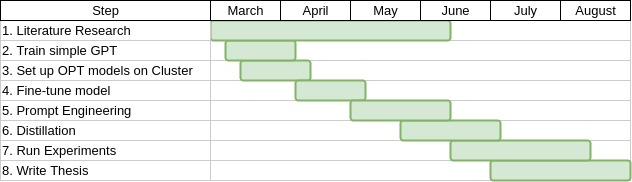
\includegraphics[width=\textwidth]{img/thesis_gantt}
    \caption{Exemplary timeline. Details are subject to change.}
\end{figure}


\paragraph{Step 1: Literature Research}
In this step, we will conduct a thorough review of the relevant literature
related to our topic. This includes reading academic articles, research papers,
and other publications to gain a better understanding of the current state of
knowledge in the field. By continuously reading relevant literature, we can
stay up-to-date with the latest advancements and incorporate them in our own
work.


\paragraph{Step 2: Train Simple GPT}
We will train a small GPT model to gain a deeper understanding of its
architecture, training procedure, and properties. By doing this, we can get
hands-on experience with the model and better understand its strengths and
limitations. This will help us to make informed decisions about how to
fine-tune larger models for our specific task.


\paragraph{Step 3: Set up OPT models on Cluster}
To run experiments later on, we need to download the model parameters and set
up the environment. It is particularly important that Multi-GPU-execution works
as expected. Additionally, we will write simple scripts to automate our later
experiments. This includes tools for evaluation, fine-tuning, and accuracy
assessment.


\paragraph{Step 4: Fine-tune model}
In this step, we will construct and train the model on select examples, with
intermediate annotations or validation in-between, similar to what is described
in \cite{dunn_structured_2022}. The first goal is to increase the task success
rate, which means answering questions in the requested machine-readable format.
The second goal is to increase accuracy. To achieve high accuracy, we may
manually annotate a few examples, and augment using partially annotated ones.


\paragraph{Step 5: Prompt Engineering}
In this step, we will apply deep introspection and automatic prompt engineering
\cite{zhou_large_2022} in an attempt to increase the accuracy of generated
databases. Prompt engineering involves designing the prompts that the model
will use to generate responses. By optimizing the prompts, we can improve the
quality of the model's output and make it more accurate.


\paragraph{Step 6: Distillation}
Distillation is a technique for reducing the size of a large model while
maintaining its accuracy. In this step, we will apply distillation
\cite{sun_patient_2019} to our model to reduce its parameter size while keeping
accuracy high. This will make the model more efficient and easier to deploy in
production.


\paragraph{Step 7: Run Experiments}
In this step, we will run detailed experiments to evaluate the performance of
our model. We will generate graphs, tables, and databases of extracted
information to analyze and interpret the results. By running experiments, we
can validate the effectiveness of our approach and identify areas for
improvement.


\paragraph{Step 8: Write Thesis}
In the final step, we will write an extensive scientific article as the
concluding work of our master's degree. This will involve summarizing our
research, detailing our methodology, presenting our results, and discussing the
implications of our findings. Writing the thesis is an essential part of the
research process and allows us to share our insights and contributions with the
broader academic community.


\bibliography{references.bib}

\end{document}
